\iffalse
\chapter{2022}
\author{AI24BTECH11022}
\section{xe}
\fi

\item The movie was funny and I \rule{1cm}{0.15mm}.\hfill(2022)
\begin{multicols}{2}
\begin{enumerate}
\item could help laughing
\item couldn't help laughed
\item couldn't help laughing
\item could helped laughed
\end{enumerate}
\end{multicols}


\item $x:y:z=\frac{1}{2}:\frac{1}{3}:\frac{1}{4}$

What is the value of $\frac{x+z-y}{y}$\hfill(2022)
\begin{multicols}{2}
\begin{enumerate}
\item $0.75$
\item $1.25$
\item $2.25$
\item $3.25$
\end{enumerate}
\end{multicols}


\item Both the numerator and the denominator of $\frac{3}{4}$ are increased by a positive
integer, $x$, and those of $\frac{15}{17}$ are decreased by the same integer. This operation
results in the same value for both the fractions.\\

What is the value of $x$?\hfill(2022)
\begin{multicols}{2}
\begin{enumerate}
\item $1$
\item $2$
\item $3$
\item $4$
\end{enumerate}
\end{multicols}


\item A survey of 450 students about their subjects of interest resulted in the
following outcome.\\

150 students are interested in Mathematics.\\
200 students are interested in Physics.\\
175 students are interested in Chemistry.\\
50 students are interested in Mathematics and Physics.\\
60 students are interested in Physics and Chemistry.\\
40 students are interested in Mathematics and Chemistry.\\
30 students are interested in Mathematics, Physics and Chemistry.\\
Remaining students are interested in Humanities.\\

Based on the above information, the number of students interested in
Humanities is\hfill(2022)
\begin{multicols}{2}
\begin{enumerate}
\item $10$
\item $30$
\item $40$
\item $45$
\end{enumerate}
\end{multicols}


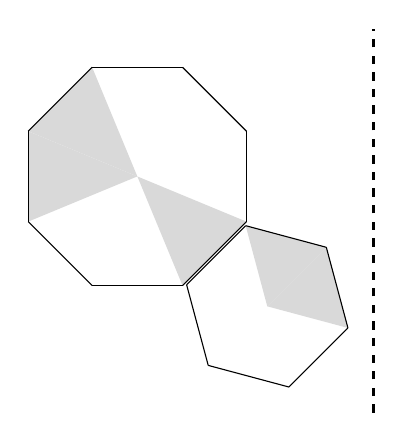
\begin{tikzpicture}[scale=0.75]
\def\radius{2}
\def\smallradius{1.414}
\foreach \angle [count=\i] in {0,45,...,315} {
\coordinate (A\i) at (\angle+22.5:\radius);
}
\foreach \i [remember=\i as \lasti (initially 8)] in {7} {
\fill[gray!30] (0,0) -- (A\i) -- (A\lasti) -- cycle;
}
\foreach \i [remember=\i as \lasti (initially 5)] in {4,3} {
\fill[gray!30] (0,0) -- (A\i) -- (A\lasti) -- cycle;
}

\foreach \i [remember=\i as \lasti (initially 8)] in {1,...,8} {
\draw (A\lasti) -- (A\i);
}
\begin{scope}[shift={(2.2,-2.2)}]
\foreach \angle [count=\i] in {0,60,...,300} {
\coordinate (B\i) at (\angle+45:\smallradius);
}
\foreach \i [remember=\i as \lasti (initially 6)] in {1,2} {
\fill[gray!30] (0,0) -- (B\i) -- (B\lasti) -- cycle;
}
\foreach \i [remember=\i as \lasti (initially 6)] in {1,...,6} {
\draw (B\lasti) -- (B\i);
}
\end{scope}
\draw[dashed,thick] (4,-4) -- (4,2.5);
\end{tikzpicture}

For the picture shown above, which one of the following is the correct picture
representing reflection with respect to the mirror shown as the dotted line?\hfill(2022)
\begin{multicols}{2}
\begin{enumerate}
\item 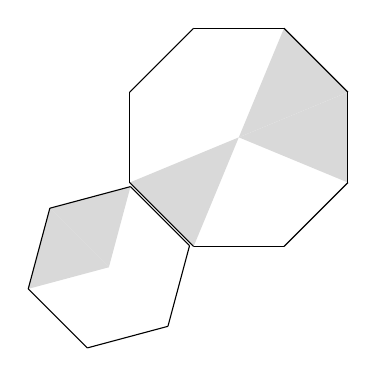
\begin{tikzpicture}[scale=0.75]
\def\radius{2}
\def\smallradius{1.414}
\foreach \angle [count=\i] in {180,225,...,495} {
\coordinate (A\i) at (\angle+22.5:\radius);
}
\foreach \i [remember=\i as \lasti (initially 1)] in {2} {
\fill[gray!30] (0,0) -- (A\i) -- (A\lasti) -- cycle;
}
\foreach \i [remember=\i as \lasti (initially 6)] in {5,4} {
\fill[gray!30] (0,0) -- (A\i) -- (A\lasti) -- cycle;
}
\foreach \i [remember=\i as \lasti (initially 8)] in {1,...,8} {
\draw (A\lasti) -- (A\i);
}
\begin{scope}[shift={(-2.2,-2.2)}]
\foreach \angle [count=\i] in {180,240,...,480} {
\coordinate (B\i) at (\angle+15:\smallradius);
}
\foreach \i [remember=\i as \lasti (initially 5)] in {6,1} {
\fill[gray!30] (0,0) -- (B\i) -- (B\lasti) -- cycle;
}
\foreach \i [remember=\i as \lasti (initially 6)] in {1,...,6} {
\draw (B\lasti) -- (B\i);
}
\end{scope}
\end{tikzpicture}
\item 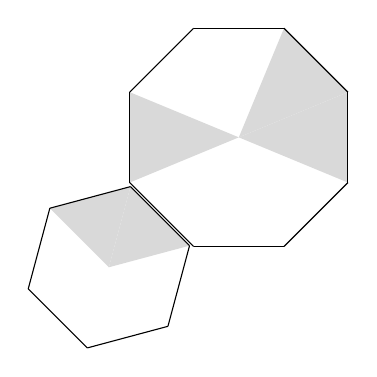
\begin{tikzpicture}[scale=0.75]
\def\radius{2}
\def\smallradius{1.414}
\foreach \angle [count=\i] in {180,225,...,495} {
\coordinate (A\i) at (\angle+22.5:\radius);
}
\foreach \i [remember=\i as \lasti (initially 1)] in {8} {
\fill[gray!30] (0,0) -- (A\i) -- (A\lasti) -- cycle;
}
\foreach \i [remember=\i as \lasti (initially 6)] in {5,4} {
\fill[gray!30] (0,0) -- (A\i) -- (A\lasti) -- cycle;
}
\foreach \i [remember=\i as \lasti (initially 8)] in {1,...,8} {
\draw (A\lasti) -- (A\i);
}
\begin{scope}[shift={(-2.2,-2.2)}]
\foreach \angle [count=\i] in {180,240,...,480} {
\coordinate (B\i) at (\angle+15:\smallradius);
}
\foreach \i [remember=\i as \lasti (initially 6)] in {5,4} {
\fill[gray!30] (0,0) -- (B\i) -- (B\lasti) -- cycle;
}
\foreach \i [remember=\i as \lasti (initially 6)] in {1,...,6} {
\draw (B\lasti) -- (B\i);
}
\end{scope}
\end{tikzpicture}
\item 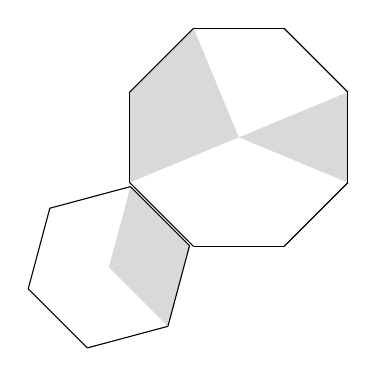
\begin{tikzpicture}[scale=0.75]
\def\radius{2}
\def\smallradius{1.414}
\foreach \angle [count=\i] in {180,225,...,495} {
\coordinate (A\i) at (\angle+22.5:\radius);
}
\foreach \i [remember=\i as \lasti (initially 4)] in {5} {
\fill[gray!30] (0,0) -- (A\i) -- (A\lasti) -- cycle;
}
\foreach \i [remember=\i as \lasti (initially 1)] in {8,7} {
\fill[gray!30] (0,0) -- (A\i) -- (A\lasti) -- cycle;
}
\foreach \i [remember=\i as \lasti (initially 8)] in {1,...,8} {
\draw (A\lasti) -- (A\i);
}
\begin{scope}[shift={(-2.2,-2.2)}]
\foreach \angle [count=\i] in {180,240,...,480} {
\coordinate (B\i) at (\angle+15:\smallradius);
}
\foreach \i [remember=\i as \lasti (initially 5)] in {4,3} {
\fill[gray!30] (0,0) -- (B\i) -- (B\lasti) -- cycle;
}
\foreach \i [remember=\i as \lasti (initially 6)] in {1,...,6} {
\draw (B\lasti) -- (B\i);
}
\end{scope}
\end{tikzpicture}
\item 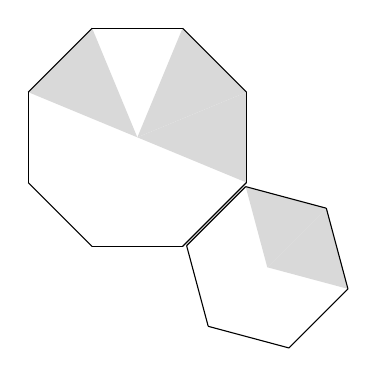
\begin{tikzpicture}[scale=0.75]
\def\radius{2}
\def\smallradius{1.414}
\foreach \angle [count=\i] in {0,45,...,315} {
\coordinate (A\i) at (\angle+22.5:\radius);
}
\foreach \i [remember=\i as \lasti (initially 4)] in {3} {
\fill[gray!30] (0,0) -- (A\i) -- (A\lasti) -- cycle;
}
\foreach \i [remember=\i as \lasti (initially 2)] in {1,8} {
\fill[gray!30] (0,0) -- (A\i) -- (A\lasti) -- cycle;
}

\foreach \i [remember=\i as \lasti (initially 8)] in {1,...,8} {
\draw (A\lasti) -- (A\i);
}
\begin{scope}[shift={(2.2,-2.2)}]
\foreach \angle [count=\i] in {0,60,...,300} {
\coordinate (B\i) at (\angle+45:\smallradius);
}
\foreach \i [remember=\i as \lasti (initially 6)] in {1,2} {
\fill[gray!30] (0,0) -- (B\i) -- (B\lasti) -- cycle;
}
\foreach \i [remember=\i as \lasti (initially 6)] in {1,...,6} {
\draw (B\lasti) -- (B\i);
}
\end{scope}
\end{tikzpicture}
\end{enumerate}
\end{multicols}


\item In the last few years, several new shopping malls were opened in the city. The
total number of visitors in the malls is impressive. However, the total revenue
generated through sales in the shops in these malls is generally low.\\

Which one of the following is the CORRECT logical inference based on the
information in the above passage?\hfill(2022)
\begin{enumerate}
\item  Fewer people are visiting the malls but spending more
\item More people are visiting the malls but not spending enough
\item More people are visiting the malls and spending more
\item Fewer people are visiting the malls and not spending enough
\end{enumerate}


\item In a partnership business the monthly investment by three friends for the first
six months is in the ratio $3:4:5$. After six months, they had to increase their
monthly investments by $10\%$, $15\%$ and $20\%$, respectively, of their initial
monthly investment. The new investment ratio was kept constant for the next
six months.\\

What is the ratio of their shares in the total profit (in the same order) at the end
of the year such that the share is proportional to their individual total investment
over the year?\hfill(2022)
\begin{multicols}{2}
\begin{enumerate}
\item $22:23:24$
\item $22:33:50$
\item $33:46:60$
\item $63:86:110$
\end{enumerate}
\end{multicols}


\item Consider the following equations of straight lines:
$$\text{Line }L1:2x-3y=5$$
$$\text{Line }L2:3x+2y=8$$
$$\text{Line }L3:4x-6y=5$$
$$\text{Line }L4:6x-9y=6$$
Which one among the following is the correct statement?\hfill(2022)
\begin{enumerate}
\item $L1$ is parallel to $L2$ and $L1$ is perpendicular to $L3$
\item $L2$ is parallel to $L4$ and $L2$ is perpendicular to $L1$
\item $L3$ is perpendicular to $L4$ and $L3$ is parallel to $L2$
\item $L4$ is perpendicular to $L2$ and $L4$ is parallel to $L3$
\end{enumerate}


\item Given below are two statements and four conclusions drawn based on the
statements.\\

Statement 1 : Some soaps are clean.\\
Statement 2 :  All clean objects are wet.\\

Conclusion \textsc{I} : Some clean objects are soaps.\\
Conclusion \textsc{II} : No clean object is a soap.\\
Conclusion \textsc{III} :  Some wet objects are soaps.\\
Conclusion \textsc{IV} : All wet objects are soaps.\\

Which one of the following options can be logically inferred?\hfill(2022)
\begin{enumerate}
\item Only conclusion \textsc{I} is correct
\item Either conclusion \textsc{I} or conclusion \textsc{II} is correct
\item Either conclusion \textsc{III} or conclusion \textsc{IV} is correct
\item Only conclusion \textsc{I} and conclusion \textsc{III} are correct 
\end{enumerate}


\item An ant walks in a straight line on a plane leaving behind a trace of its
movement. The initial position of the ant is at point $P$ facing east.\\

The ant first turns $72\degree$ anticlockwise at $P$, and then does the following two
steps in sequence exactly FIVE times before halting.\\

1. moves forward for $10cm$.\\
2. turns $144\degree$ clockwise.\\

\begin{tikzpicture}
\draw[->] (0,-1) -- (0,1) node[above] {North};
\draw[->] (-1,0) -- (1,0) node[right] {East};
\end{tikzpicture}

The pattern made by the trace left behind by the ant is\hfill(2022)
\begin{enumerate}
\item 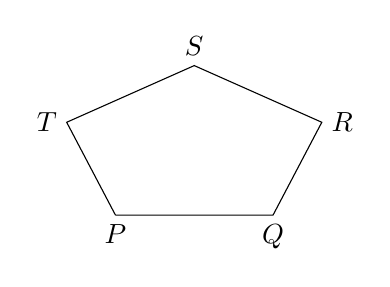
\begin{tikzpicture}
\draw (-1,0) node[left,below] {$P$} -- (1,0) node[right,below] {$Q$} -- (1.62,1.18) node[right] {$R$} -- (0,1.9) node[above] {$S$} -- (-1.62,1.18) node[left] {$T$} -- (-1,0);
\end{tikzpicture} $PQ=QR=RS=ST=TP=10cm$
\item 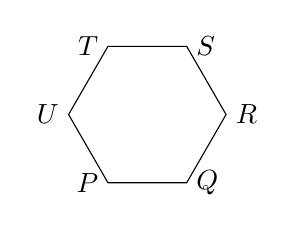
\begin{tikzpicture}
\draw (-0.5,-0.866) node[below,left] {$P$} -- (0.5,-0.866) node[below,right] {$Q$} -- (1,0) node[right] {$R$} -- (0.5,0.866) node[above,right] {$S$} -- (-0.5,0.866) node[above,left] {$T$} -- (-1,0) node[left] {$U$} -- (-0.5,-0.866);
\end{tikzpicture} $PQ=QR=RS=ST=TU=UP=10cm$
\item 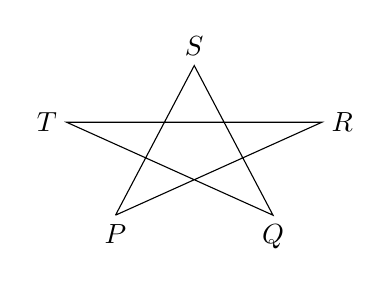
\begin{tikzpicture}
\draw (-1,0) node[left,below] {$P$} -- (1.62,1.18) node[right] {$R$} -- (-1.62,1.18) node[left] {$T$}  -- (1,0) node[right,below] {$Q$}  -- (0,1.9) node[above] {$S$} -- (-1,0);
\end{tikzpicture} $SQ=QT=TR=RP=PS=10cm$
\item 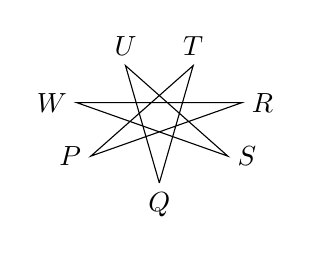
\begin{tikzpicture}
\draw (0,0) node[below] {$Q$} -- (0.43,1.49) node[above] {$T$} -- (-0.87,0.34) node[below,left] {$P$} -- (1.05,1.02) node[right] {$R$} -- (-1.05,1.02) node[left] {$W$} -- (0.87,0.34) node[below,right] {$S$} -- (-0.43,1.49) node[above] {$U$} -- (0,0);
\end{tikzpicture} $SW=WR=RP=PT=TQ=QU=US=10cm$
\end{enumerate}


\item The value of $\lim_{x\rightarrow 0}\frac{1}{x}\int_{2}^{2+x}\brak{t+\sqrt{t^{2}+5}}dt$ is\hfill(2022)
\begin{multicols}{2}
\begin{enumerate}
\item $0$
\item $4$
\item $5$
\item $6$
\end{enumerate}
\end{multicols}


\item Let $\mathbb{C}=\cbrak{z=x+iy:x\text{ and }y\text{ are real numbers, }i=\sqrt{-1}}$ be the set of complex numbers. Let the function $f\brak{z}=u\brak{x,y}+iv\brak{x,y}$ for $z=x+iy\in\mathbb{C}$ be analytic in $\mathbb{C}$, where $$u\brak{x,y}=xy^{3}-yx^{3}\text{ and }v\brak{x,y}=\frac{x^{4}}{4}+\frac{y^{4}}{4}-\frac{3}{2}x^{2}y^{2}$$ If $f^{\prime}\brak{z}$ denotes the derivative of $f\brak{z}$, then\hfill(2022)
\begin{multicols}{2}
\begin{enumerate}
\item $\abs{f^{\prime}\brak{-1+i}}^{2}=1$
\item $\abs{f^{\prime}\brak{-1+i}}^{2}=7$
\item $\abs{f^{\prime}\brak{-1+i}}^{2}=8$
\item $\abs{f^{\prime}\brak{-1+i}}^{2}=10$
\end{enumerate}
\end{multicols}


\item If the partial differential equation $$\brak{x+2}\frac{\partial^{2}u}{\partial x^{2}}+2\brak{x+y}\frac{\partial^{2}u}{\partial x\partial y}+2\brak{y-1}\frac{\partial^{2}u}{\partial y^{2}}-3y^{2}\frac{\partial u}{\partial y}=0$$ is parabolic on the circle $\brak{x-a}^{2}+\brak{y-b}^{2}=r^{2}$, then the values of $a$, $b$ and $r$ are given by\hfill(2022)
\begin{multicols}{2}
\begin{enumerate}
\item $a=1,b=2,r=1$
\item $a=-1,b=2,r=1$
\item $a=1,b=-2,r=1$
\item $a=-1,b=-2,r=1$
\end{enumerate}
\end{multicols}